% !TeX root = ../main.tex

\chapter{數值模型}

同第一章所述,地球動力學為探討地球內部的動力過程,以及地球內部物質受力後所發生的變形作用,其所牽扯的運動過程複雜。
地質學藉由地表觀察,可得知過去地表上經歷的地質事件,進而間接獲得當時的動力狀態,不過隨著時間推移,可用的岩石紀錄越來越少,並且地質資料並無法完全代表地球內部的動力過程。
地球內部的直接觀察僅能靠鑽井資料獲取,然而地球上最深的鑽井資料為12公里(\citealp{ganchin1998seismic}),不到地球半徑的千分之二。
因此,只能靠間接方法探測地球內部,地球物理學便是強大研究學門。
地球物理學包含多種研究,重力學、磁力學、大地電磁等方法利用矩陣逆推(inversion)計算地表測站資料,獲得地下構造成像,不過這些方法並不是接收直接通過地球內部介質而來的訊號,因此約束不多且深度解析有限。
地震波能量穿透整個地球被全球地表測站接收,過程中地震波直接通過地球內部介質,為地球內部構造提供有效的資訊,固地震學為目前最常見對地球深部構造的探勘方法。
儘管如此,最早的地震學發展始於19世紀末,其所觀測得之構造在地質時間尺度上只能被視為瞬間狀態,無法代表地球內部過去的構造狀態。
為了彌補地球內部在時間上與空間上的有限數據量,地質建模與模擬成為探討地球內部演化的有力工具。

在本研究的數值模型中,地球動力學所牽扯的運動過程複雜,不適用單純的質點或剛體運動,需要使用連續體力學(Continuum mechanics)的物理概念描述岩石的動力與變形行為。
在模型中將岩石單元視為地質構造上的連續介質(Continuum media),岩石具有巨觀物理量,受牛頓力學所支配,系統中的總力除了質點運動中所包含的外力(external force)之外,還需要考慮系統的內部作用力(internal force)。
連續介質特性描述可被用於岩石的密度、壓力、速度、應變等不同維度物理的場變量(field variables)。
由於在地質尺度上長期且緩慢的岩石變形過程可視為流體,因此地球動力學模型在不同尺度上部分可視為流體力學的展現。
而流體力學的數學式共有三大守恆定律,分別為質量守恆、動量守恆與能量守恆。
該三大守恆定律可寫成偏微分方程式的形式,同時也是連續方程式,此時因偏微分方程式之解析解多半不存在,僅能利用數值近似方法求得最佳解。

在本章節中會介紹數值模擬的計算方式以及模型物質物理特性。

\section{FLAC}

本研究使用Fast Lagrangian Analysis of Continua (FLAC,快速拉格朗日連續體分析) 技術,最早是由\citealp{cundall1989numerical}開發的二維顯性(explicit)有限差分(Finite Difference Method, FDM)數值分析程式。
爾後由\citealp{Lavier2000}改良,適用於模擬地球動力與地球內部變形。
FLAC使用拉格朗日描述法(Lagrangian formulation)與非均值網格(structured non-uniform mesh),在符合牛頓力學的情況下,於每個時間段上求解每個節點(node)的運動方程式,算出每個節點上所受到的力,計算出新的速度與位移,獲得節點應變,再藉由岩石流變學物性方程式(constitutive equation)從應變推得節點所受應力,作為下一時間的初始作用力,流程見圖\ref{fig::FLAC_method}。

\begin{figure*}[ht!]
    \centering
    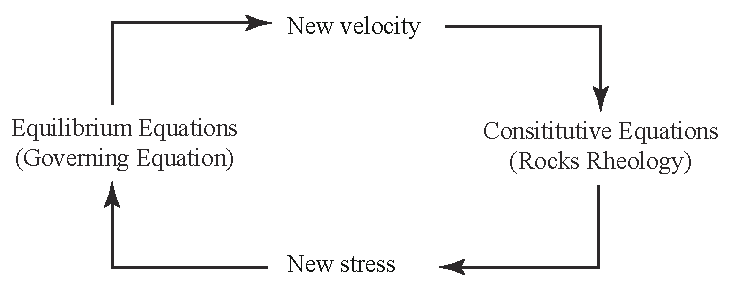
\includegraphics[width=4in]{FLAC_flow.pdf}
    \caption[FLAC 程式運算流程圖]{FLAC 程式運算流程圖。}
    \label{fig::FLAC_method}
\end{figure*}
單一網格中存在一定數量的標記點(marker),紀錄岩相、位置等特徵,標記點的速度由計算獲得的速度決定,可在網格間移動。
由於模型中的網格會根據所受的應力變形,在一段時間內若網格扭曲嚴重、網格的邊界角度過大或過小,則FLAC會重建網格,該過程稱為網格重建(remesh)。
此時所有網格與節點會重新排列,並使用差分標記點上的物理量獲得新節點的物理量。

FLAC所使用的主控方程式包含質量守恆、動量守恆與能量守恆方程式。考量岩石流變學中的彈性、塑性與黏性變形行為,以下將一一介紹主控方程式與岩石流變學。
\section{主控方程式}

\subsection{質量守恆}
由於FLAC使用拉格朗日描述法,每個拉格朗日點被嚴格的連到一單一的物質點上,並且會隨著該點移動。
因此,同一個質點總是在同一座標上,與時間無關,該座標滿足質量守恆。
拉格朗日描述法的質量守恆方程式如下:
\begin{align}
\frac{D\rho}{Dt}+\rho\nabla\cdot\vec v =0 
\label{eqn:MASS_Lagrangian}
\end{align}
其中 $\frac{D\rho}{Dt}$ 表示拉格朗日座標下的密度隨時間變化,$\rho$為密度,$\vec v$為速度向量。

\subsection{動量守恆}
地球內部的動力包含了介質所受之外力與內力力平衡的結果,並且在物質受力後產生變形。
在數值計算中利用動量守恆方程式將力與變形聯繫,滿足牛頓第二運動定律。
\begin{align}
\vec f=m\vec a
\end{align}
$f$ 為作用在物質上的作用力,$m$為物質的質量。
本研究所使用之拉格朗日坐標系下動量守恆方程式為:
\begin{align}
\rho \frac{ Dv_{i}}{Dt} = \frac{\partial \sigma_{ij}}{\partial x_j}+\rho g_i\label{eqn:momentum Lagrangian}
\end{align}
或
\begin{align}
\rho \vec a = \nabla\cdot\vec\sigma+\rho\vec g\label{eqn:momentum Lagrangian2}
\end{align}
此為Navier-Stokes方程式。 其中$\rho$為密度,$\vec a$為節點加速度,$\vec\sigma$為應力張量(stress tensor),$g$為重力加速度。

\subsection{能量守恆}
為了描述一連續體中的能量平衡狀態,使用溫度方程式表示能量的進出。
拉格朗日描述法下的能量守恆方程式表示如下:
%\begin{align}
%\rho C_p \frac{DT}{Dt} = -\frac{\partial q_x}{\partial x}-\frac{\partial q_y}{\partial y}-\frac{\partial q_z}{\partial z}+H_s+H_L
%\end{align}
%將熱通量拆解:
%\begin{align}
%q=-k\frac{\partial T}{\partial x}
%\end{align}
\begin{align}
\rho C_p \frac{DT}{Dt} = k\nabla^2T+H_s+H_L
\label{eq:heat equation}
\end{align}
式\ref{eq:heat equation}為拉格朗日座標下標準的熱擴散方程式加上額外的兩種熱源,分別為摩擦熱($H_s$, friction heat)與潛熱($H_L$, latent)。
其中$T$是溫度,$\rho$是密度,$C_p$是等壓比熱容量,$k$是熱傳導係數。
摩擦熱($H_s$)由剪切力在不可逆變形中能量耗散所產生,通式如下:
\begin{align}
    H_s = \sigma^{'}_{ij}\dot\varepsilon^{'}_{ij}
\end{align}
$\sigma^{'}$為軸差應力(deviatoric stress),$\dot\varepsilon^{'}$為軸差應變率(deviatoric strain rate)。

潛熱($H_L$)為物質發生相態變化過程中,溫度不變時釋放或吸收的能量,本研究唯一有考慮的潛熱為岩漿結晶中產生的放熱,在\ref{岩漿作用造成的溫度影響}節中有較詳細的介紹。
本研究中並沒有考慮放射性元素所產生的熱。
主控方程式沒有考慮絕熱(adiabatic)溫度梯度,因此動力過程中的溫度皆不包含絕熱溫度,然而本研究在不影響動力過程的相變與岩漿作用下有考慮絕熱溫度梯度。

\section{岩石流變學}
主控方程式包含七個方程式與十個未知數,因此求解過程需要額外方程式。
岩石的流變學由物性方程式所表示,不同的岩石具有不同物理性質。

在近地表區域,岩石處於相對較低溫的環境,因此地球岩石圈表層由脆性變形(brittle deformation)所主導,包含低壓下的彈性變形(elastic deformation)與高壓下的塑性變形(plastic deformation)。
而在地球岩石圈深處到地球內部,岩石因周遭溫度隨深度增加而表現出不可逆的黏性變形(viscous deformation)。
因此,若地球動力學模型需同時考慮廣泛的岩石變形特性時,則模型流變學應同時包含彈-塑-黏性(elasto-visco-plastic)變形。

彈性變形假設物質所承受的應力與其應變呈正比,可以是虎克定律的展現。彈性變形很重要的精隨為其變形是可逆的,若施加在彈性物質上的應力被移除,其變形量會變回零。
由虎克定律得到彈性通式:
\begin{align}
\sigma_{ij}=E_{ijkl} \varepsilon_{kl}
\end{align}
其中,$\sigma$為二階應力張量(stress tensor),$E$為四階張量彈性常數(elastic constant),$\varepsilon$為應變。
假設物質具有均質性(isotropic),則上列通式矩陣僅會有兩個獨立分量:

\begin{align}
    \sigma_{ij}=\lambda_1 \varepsilon_{kk} \delta_{ij}+2 \lambda_2 \varepsilon_{ij}=K\varepsilon_{kk} \delta_{ij}+2 \mu \varepsilon_{ij}^{'} \label{eqn:elastic tensor}
\end{align}
這裡的$\sigma_{ij}$為本研究所使用的彈性應力$\sigma_{elastic}$。

彈性力學所使用的拉梅參數為$\lambda_1 = \lambda_2 = 3 \times 10^{10} Pa$,$\varepsilon^{'}$為軸差應變,其中第一拉梅參數(Lamé's first parameter, $\lambda_1$)與體彈性系數(bulk modulus, $K$)、剪彈性系數(shear modulus, $\mu$)的關係式如下:
\begin{align}
\lambda_1 = K - \frac{2}{3}\mu
\end{align}

第二拉梅參數(Lamé's second parameter, $\lambda_2$)等同於剪彈性系數。

本研究所使用的塑性變形滿足莫爾庫倫破壞準則(Mohr-Coulomb)定義屈服應力(yield stress)大小:
\begin{align}
    \sigma_{yield}=C+tan(\phi)\sigma_{n}\label{eqn:plastic deformation}
\end{align}
這裡的屈服應力(yield stress)等同本研究中的塑性應力$\sigma_{plastic}$。
其中$C$為內聚力,$\sigma_n$為正向力,$\phi$為物質摩擦角。
當物質不可逆變形(破壞)發生後,達到再次破壞變形所需的應力會大幅下降,這是物質應力弱化(strain weakening)的展現,其內部內聚力與摩擦角皆會降低,伴隨著物質強度降低。
本研究中假設已破壞物質之內聚力與摩擦角會線性降低直到一飽和最小值,如圖\ref{fig::plastic_deformatiom},表示發生過破裂的物質強度變弱。
岩石摩擦角與內聚力的值會隨應變率從0到$\varepsilon_{pl,saturate}$之間在($C_0$, $\phi_0$)與($C_1$, $\phi_1$)之間線性遞減,隨後達到摩擦角與內聚力的飽和最小值。
本研究各物質所使用的內聚力與摩擦角見表\ref{table::phase_table}。
\begin{figure*}[ht!]
    \centering
    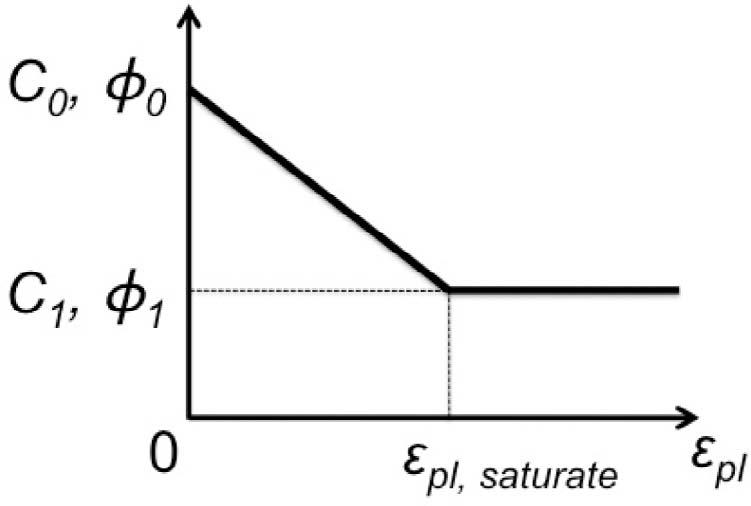
\includegraphics[width=3in]{Tan 2012 plastic.jpg}
    \caption[應力弱化示意圖,摘自\citealp{Tan2012}]{應力弱化示意圖,摘自\citealp{Tan2012}。在應變率為$0$時,岩石摩擦角與內聚力分別為$C_0$, $\phi_0$;在應變率大於$\varepsilon_{pl,saturate}$時,岩石摩擦角與內聚力分別為$C_1$, $\phi_1$。摩擦角與內聚力的值會隨應變率變化在($C_0$, $\phi_0$)與($C_1$, $\phi_1$)之間線性遞減。
    }
    \label{fig::plastic_deformatiom}
\end{figure*}

最終採用的彈塑性應力$\sigma_{elasto-plastic}$依照彈性應力($\sigma_{elastic}$)與塑性應力($\sigma_{plastic}$)的量值決定,共可分為兩種情形:

1. 若$\sigma_{elastic} <= \sigma_{plastic}$,則$ \sigma_{elasto-plastic} = \sigma_{elastic}$,物質不發生破壞。

2. 若$\sigma_{elastic} > \sigma_{plastic}$, 則物質發生破壞,需將$\sigma_{elastic}$投影至屈服面上以獲得物質發生破壞最小所需應力$\sigma_{elasto-plastic}$ (\citealp{simo2006computational})。

當溫度較高,材料強度相對進地表較低,以黏彈性(visco-elastic)變形為主。
本研究使用實驗結果所得的非牛頓流體位錯蠕變定律(dislocation creep laws)定義岩石黏滯度(\citealp{Chen1990}):
\begin{align}
   \eta=\frac{1}{4}(\frac{4}{3A})^{\frac{1}{n}} \dot\varepsilon_{II}^{' \frac{1-n}{n}} exp(\frac{E}{nR(T+273)})
   \label{eqn:viscousity}
\end{align}
$\eta$為黏滯度,$\dot\varepsilon^{'}$為軸差應變率張量矩陣,$\dot\varepsilon_{II}^{'}$為軸差應變率張量矩陣的第二不變量,$n$為應力冪數(stress exponent),$A$為材料的指數前因子(viscosity pre-exponent),$T$為攝氏溫度,$E$為活化能(activation energy),$R$為氣體常數(universal gas constant),本研究各物質所使用的應力冪數、材料的指數前因子與活化能見表\ref{table::phase_table}。
由於黏滯度會隨溫度升高而降低,本研究中,施加一臨界黏滯度最小值至10$^{20}$ Pa$\cdot$s,以防止黏滯度過低導致計算量過大。
黏彈性應力與黏滯度、應變率成正比,其計算方式如下:	
\begin{align}
    \sigma_{viscous} = 2\eta\dot\varepsilon^{'} \label{eqn:viscous tensor}
\end{align}
最終採用的黏彈性應力$\sigma_{elasto-viscous}$為馬克士威模型(Maxwell model),其為一純黏性阻尼與純彈性彈簧串連組成。

在同一網格中會分別計算每個網格上的$\sigma_{elasto-plastic}$與$\sigma_{elasto-viscous}$,每個網格所採計的應力值為($\sigma_{elasto-plastic}$, $\sigma_{elasto-viscous}$)兩者之間的最小值。
模型的岩石強度剖面示意圖如圖$\ref{fig::strength}$所示。
\begin{figure*}[ht!]
    \centering
    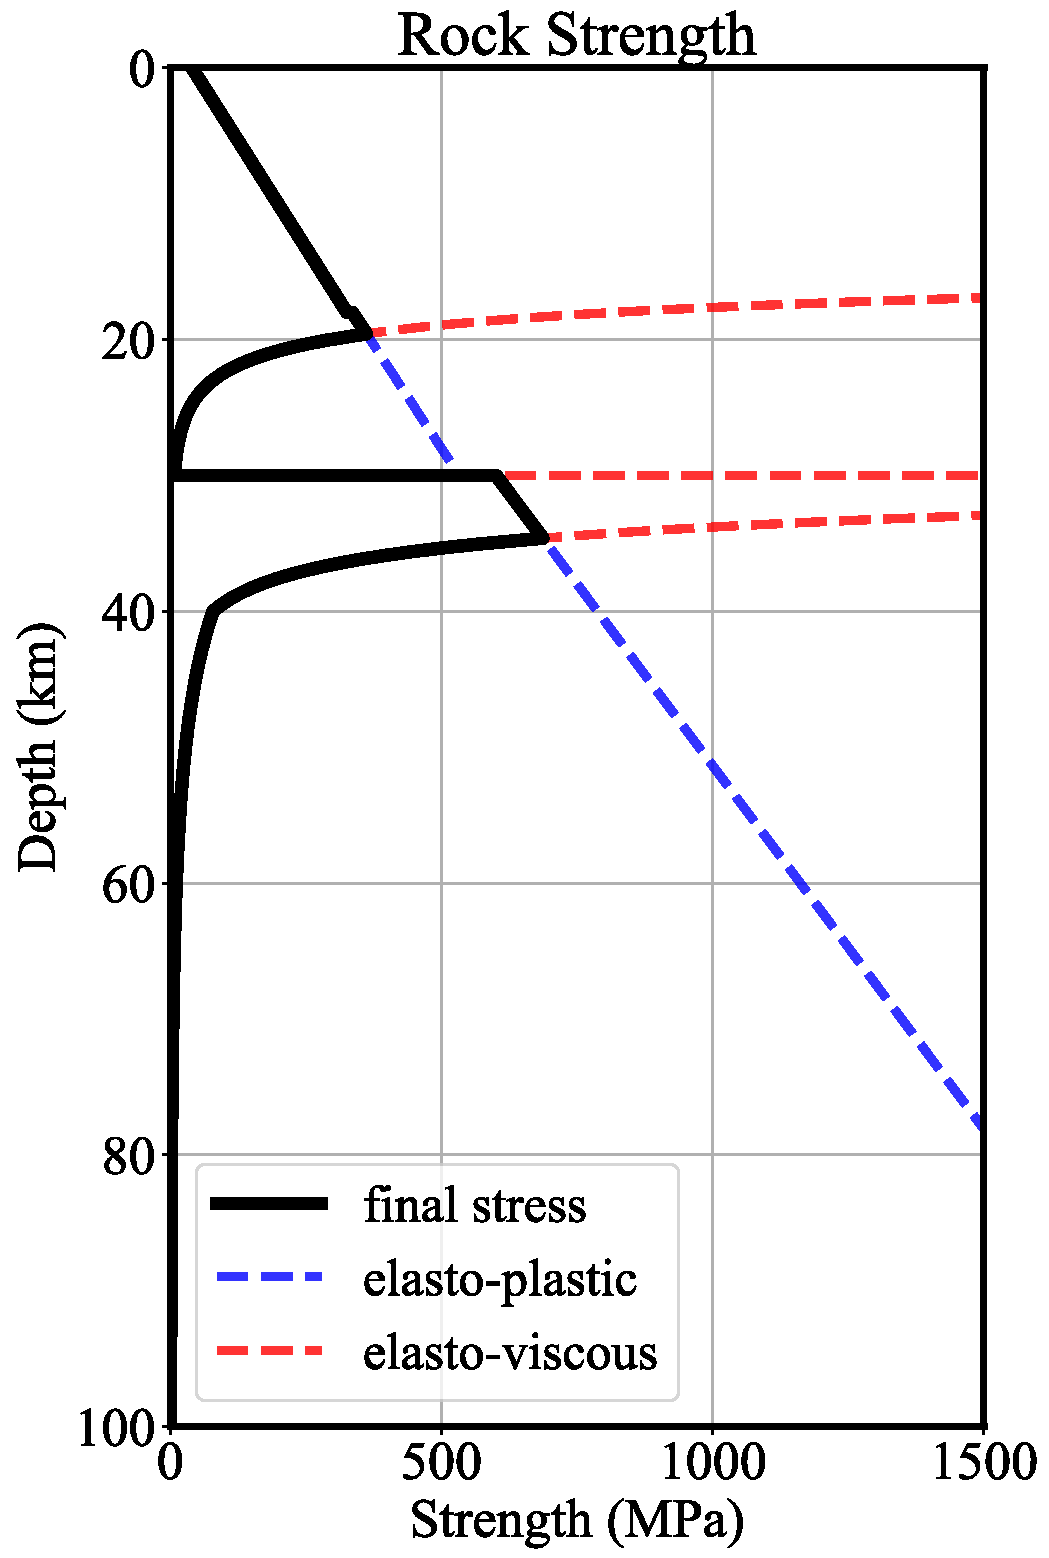
\includegraphics[height=3in]{strength_v3.pdf}
    \caption[岩石強度剖面示意圖]{岩石強度剖面示意圖,藍色虛線為彈塑性變形;紅色虛線則為黏彈性變形。黑色實線為最終強度,採用$\sigma_{elasto-plastic}$, $\sigma_{elasto-viscous}$兩者之間最小值。}
    \label{fig::strength}
\end{figure*}

\section{相變}\label{相變}

為了模擬自然界中岩石動力學中的物理性質變化,本研究考慮部分岩石相變機制,利用岩石溫度壓力狀態當作簡單相變條件。
考量相變過程可以讓隱沒模型之運動況狀以更真實的型態呈現,更能真實展現隱沒帶中力學分配過程。

在本研究中,使用模型中的標記點追蹤物質之岩相與位置,一旦所在網格之溫度與壓力滿足標記點物質之相變條件,則會判定該標記點發生相變,其岩相轉換為相變後之新岩相。
相變完成後,標記點物質所有物理性質皆會從原先岩相之性質轉變成新岩相之性質。
由於相變過程不影響運動狀態,但與溫度相關,因此模型中在考慮相變時,該位置溫度會將絕熱溫度梯度加回模型的溫度中。
以下將一一列出模型中所考慮的相變過程。

\subsection{蛇紋岩化的橄欖岩}\label{蛇紋岩化的橄欖岩}
一旦隱沒板塊進入地函中,隱沒海洋板塊上之沉積物在高溫高壓下會釋放大量流體至楔中,絕大部分集中在地函楔。乾的地函楔因而經歷水合作用,導致部分橄欖岩被蛇紋岩化。
蛇紋岩化橄欖岩(serpentinized peridotite)在這裡又稱為蛇紋岩(serpentinite),主要集中於隱沒帶中淺部,並且目前人類對於蛇紋岩之相變作用尚未有高度不確定性,因此本研究中以參數化方式模擬蛇紋岩相變過程。
使用者可自行調整在隱沒板塊上方有多少厚度的地函楔會因脫水作用相變成蛇紋岩(\citealp{Tan2012}),見圖\ref{fig::serpeninite_parameter}。
在本研究中,蛇紋岩之岩相物理性質約略等同於橄欖岩中有百分之15之橄欖岩被蛇紋岩化,過去的實驗指出其相比於橄欖岩,活化能大幅減少(\citealp{hilairet2007high}),因此蛇紋岩強度極弱,遠小於普通地函。

\begin{figure*}[ht!]
    \centering
    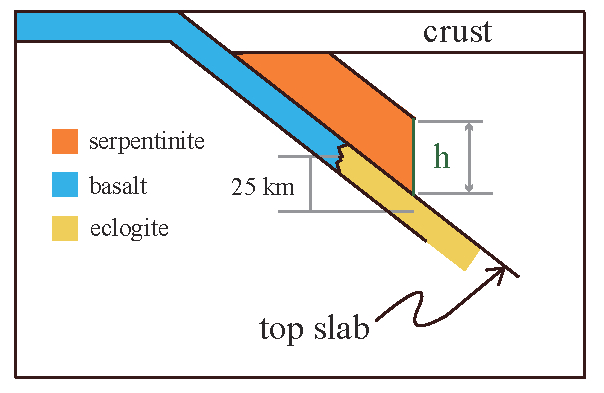
\includegraphics[width=4in]{serpeninite_parameter.pdf}
    \caption[蛇紋岩參數化示意圖]{蛇紋岩參數化示意圖。於模型隱沒板塊上,海洋地殼玄武岩相變成榴輝岩深度後25公里深之上的地函會生成h公里厚的蛇紋岩。}
    \label{fig::serpeninite_parameter}
\end{figure*}

蛇紋岩將隱沒帶流體帶入更深的地函中後,約在80-120公里之間再次發生脫水將水分釋放至地函楔中。
本研究中,在符合以下溫壓條件時(\citealp{Ulmer1995}),該脫水作用成立,蛇紋岩將相變回橄欖岩:
\begin{align}
P > 2.1 + (7.5-2.1)\times (T-730)/(500-730) \quad GPa \\
P > 2.1 + (0.2-2.1) \times (T-730)/(650-730) \quad GPa
\end{align}
其中$T$為攝氏($^\circ C$)。
圖\ref{fig::serpentinite_phase_diagram}為橄欖岩相溫壓相圖。
\begin{figure*}[h!]
    \centering
    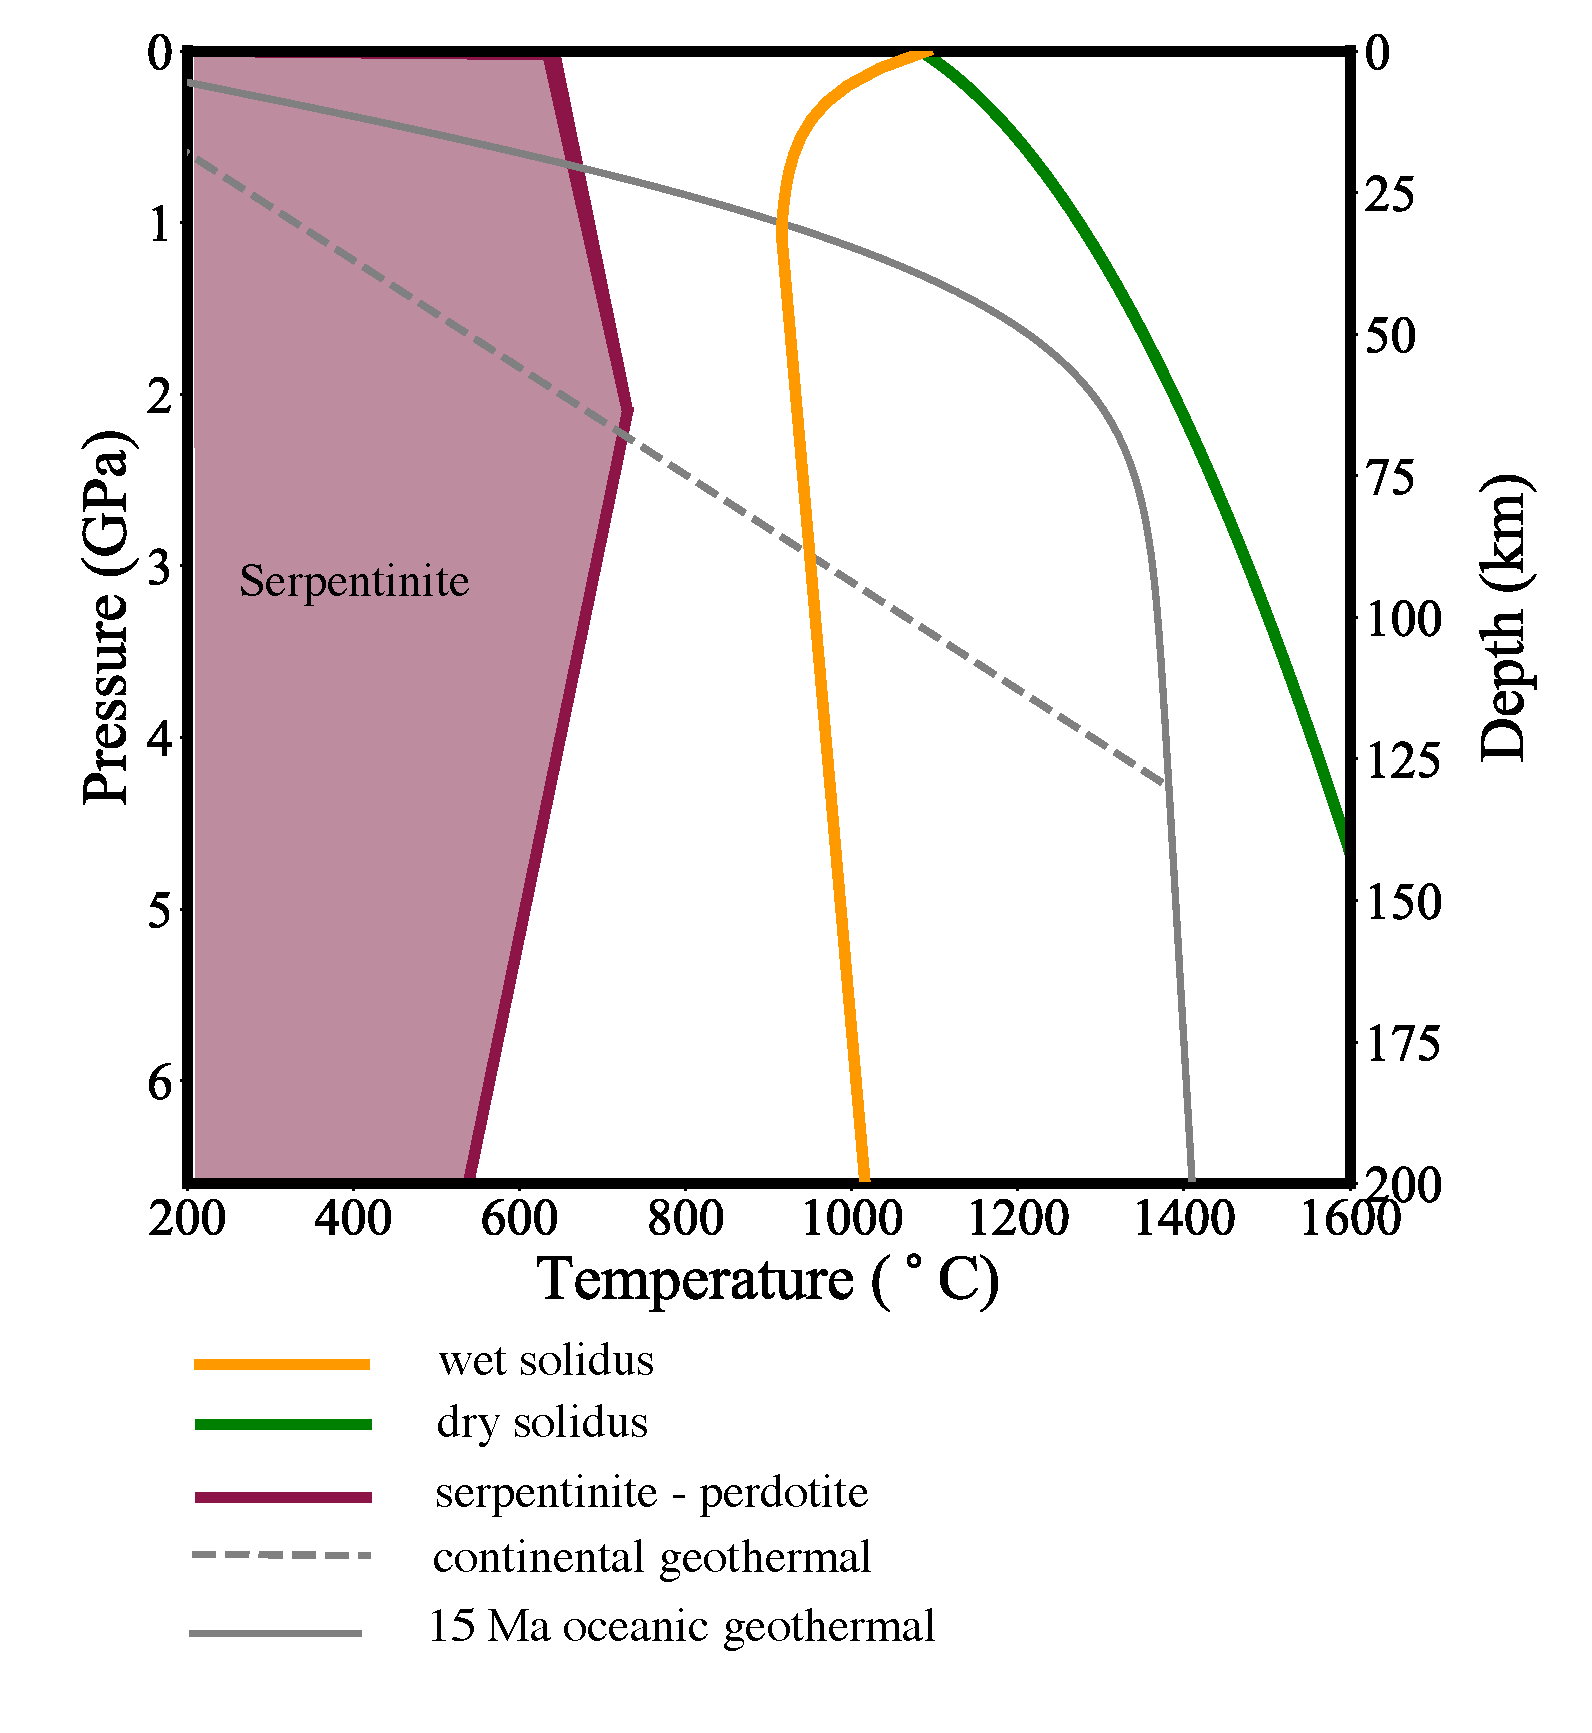
\includegraphics[width=4in]{serpentinite_phase_diagram_v1.pdf}
    \caption[橄欖岩相圖,參考\citealp{Ulmer1995}]{橄欖岩相圖。紫線代表蛇紋岩脫水回橄欖岩之相變圖,參考\citealp{Ulmer1995};綠線與黃線分別代表橄欖岩的乾固相線(dry solidus)與含水固相線(wet solidus),摘自\citealp{katz2003new}。另用灰線實線與虛線分別表示墨西哥參考模型之海洋岩石圈與大陸岩石圈地溫梯度。}
    \label{fig::serpentinite_phase_diagram}
\end{figure*}

本研究所使用的橄欖岩含水固相線(wet solidus)參考自\citealp{katz2003new},簡化式如下。
\begin{align}
    T > max (980+6\times (3.3 \times P-14) ,\quad 1090-178\times(1-exp(-4.125\times P))) ^\circ C 
\end{align}
其中$P$為十億帕斯卡(GPa)。

\subsection{玄武岩 --- 榴輝岩}

隨著隱沒板塊沉入更深的地函,其上的鎂鐵質玄武岩在高壓條件下進入榴輝岩穩定場,此時發生玄武岩相變,由高溫高壓實驗可獲得穩定場溫壓界線(\citealp{Hacker2003}),詳見下圖鎂鐵質岩相圖\ref{fig::basalt_phase_diagram}。
榴輝岩在隱沒帶中扮演非常重要的角色,同第一章所提及,榴輝岩是變質岩相中密度最大的相,造成的重力效應可以維持隱沒帶的持續性,為板塊拉力(slab pull)的驅動力。
在模型中,網格內的標記子會追蹤玄武岩海洋地殼的溫壓狀態,並與榴輝岩穩定性場進行了比較,以下方程為鎂鐵質玄武岩相變的簡化條件式。

\begin{align}
    P > 0.0022 \times T -0.3  \quad GPa\\
    P > -0.0375 \times T + 20.1  \quad GPa
\end{align}
其中$T$為攝氏($^\circ C$)

此外,本研究亦考慮鎂鐵質岩的部分熔融(partial melting)作用,鎂鐵質岩的含水固相線參考自\citealp{Gutscher2000Bcan},簡化式如下。
\begin{align}
    T > 1050-420 \times (1-exp(-P\times 3.3)) \; ^\circ C \quad if \; P <= 1 \; GPa\\
    T > 630 + 13 \times (-P)^2\; ^\circ C \quad if \; 1 < P <= 2.6 \;GPa 
    %T > 43\times(P+14)\; ^\circ C \quad if \; P > 2.6\; GPa
\end{align}
圖\ref{fig::basalt_phase_diagram}為鎂鐵質岩相溫壓相圖。
\begin{figure*}[ht!]
    \centering
    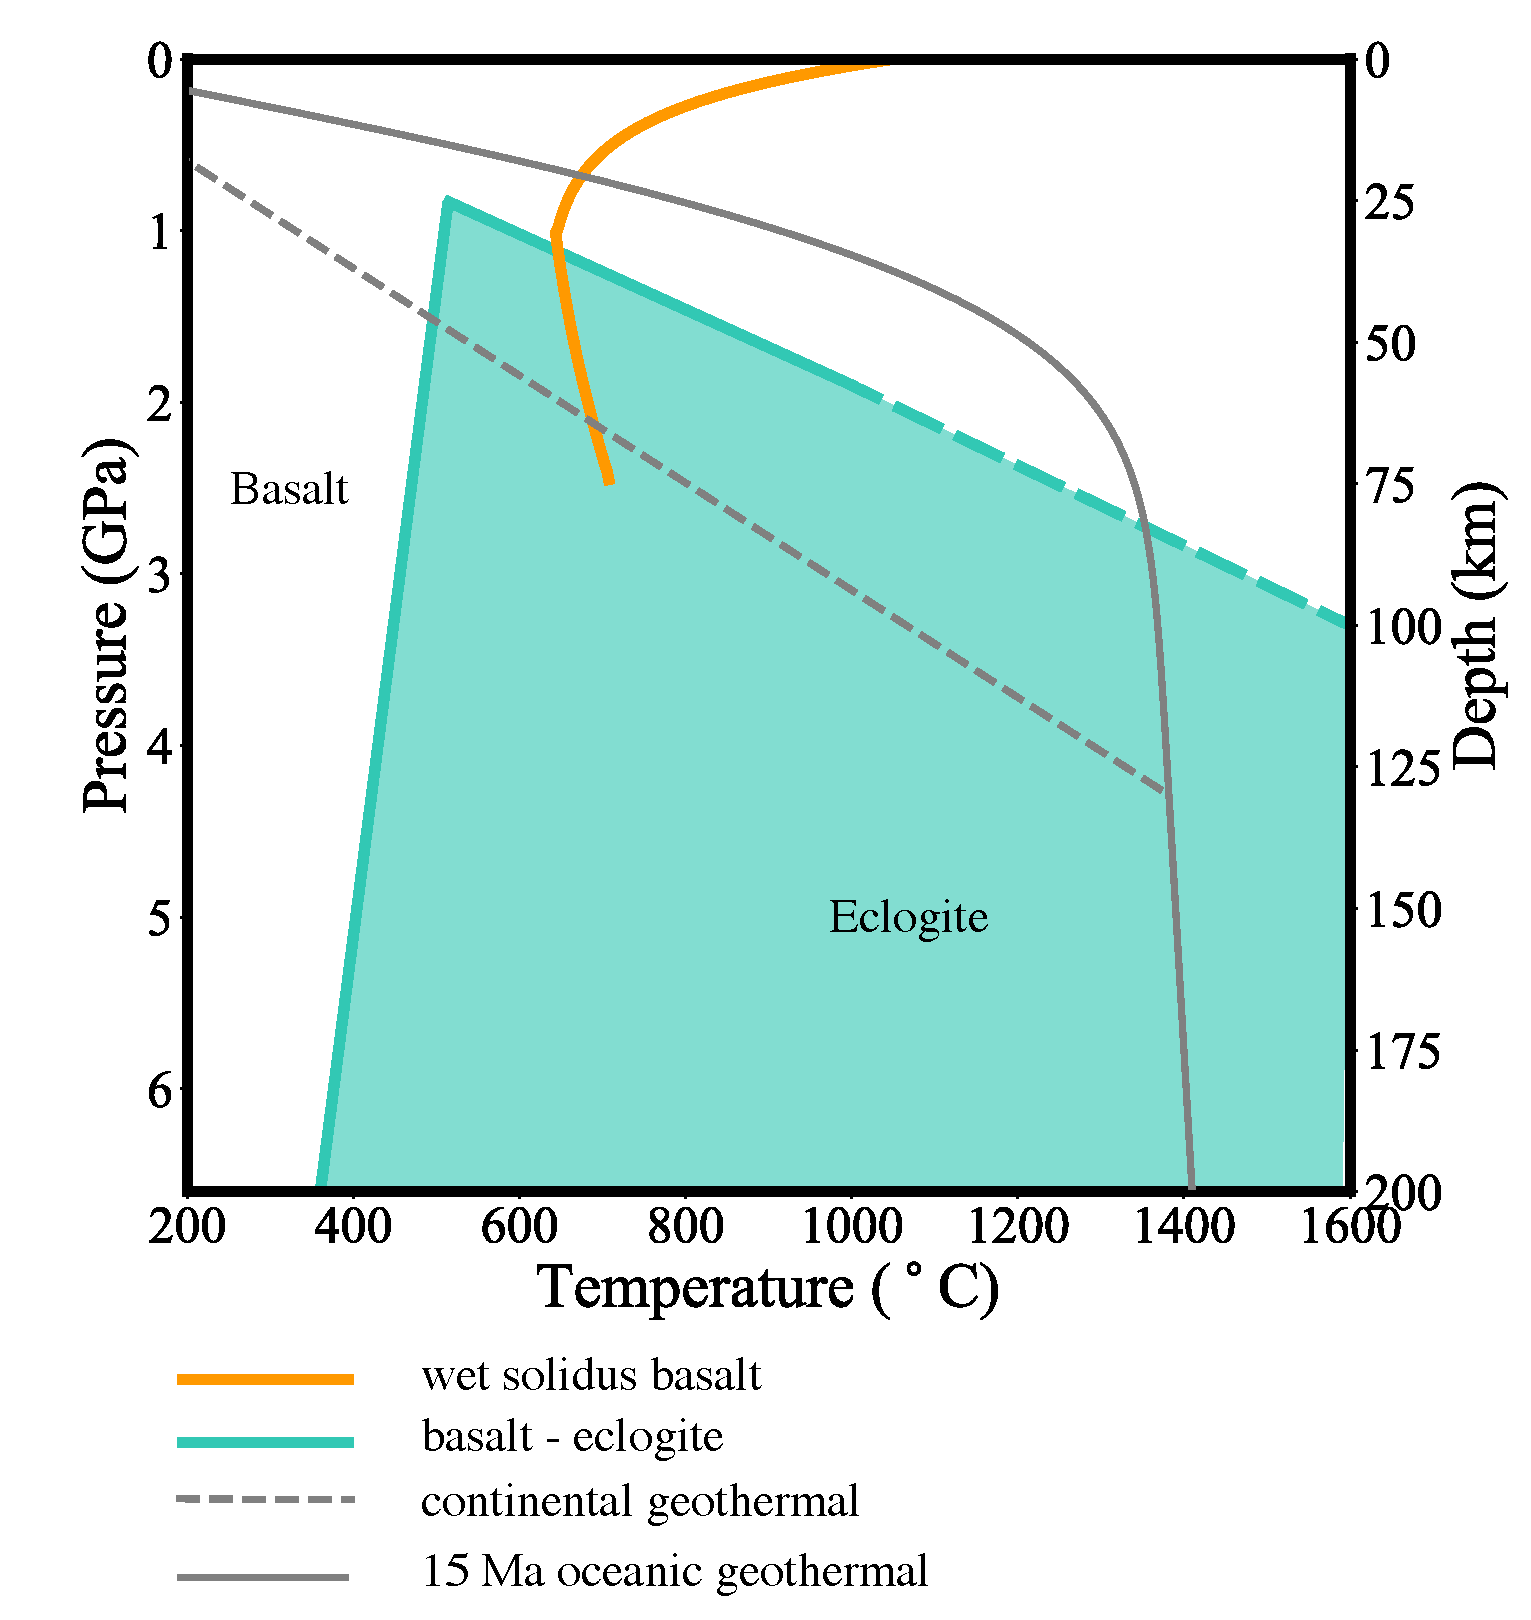
\includegraphics[width=4in]{basalt_phase_diagram_v1.pdf}
    \caption[鎂鐵質岩相圖,參考自\citealp{Hacker2003}與\citealp{Gutscher2000Bcan}]{鎂鐵質岩相圖,綠線隔開玄武岩與榴輝岩的穩定場,參考自\citealp{Hacker2003},橘線為鎂鐵質岩的含水固相線,參考自\citealp{Gutscher2000Bcan},綠虛線為外插值。}
    \label{fig::basalt_phase_diagram}
\end{figure*}

\subsection{沉積岩 --- 片岩}
模型中的沉積物在隱沒過程中進入高壓環境,發生成岩作用、壓密作用與變質作用。
不過由於這一系列作用是連續的,因此模型中的相變過程並不會造成岩石有大幅度物理性質上的改變。
下列方程為沉積物轉為片岩過程的條件式。
\begin{align}
T > 650\; ^{\circ} C
\end{align}
本研究有考量沉積物的部分熔融,參考自\citealp{van2011subduction}。
\begin{align}
    T > max (578+ P \times 0.121,\ 617+e^{P\times 1.7\times 10^{-3}}) \; ^{\circ} C
\end{align}
其中$P$為十億帕斯卡(GPa)。
圖\ref{fig::sediment_phase_diagram}為沉積物岩相溫壓相圖。
\begin{figure*}[ht!]
    \centering
    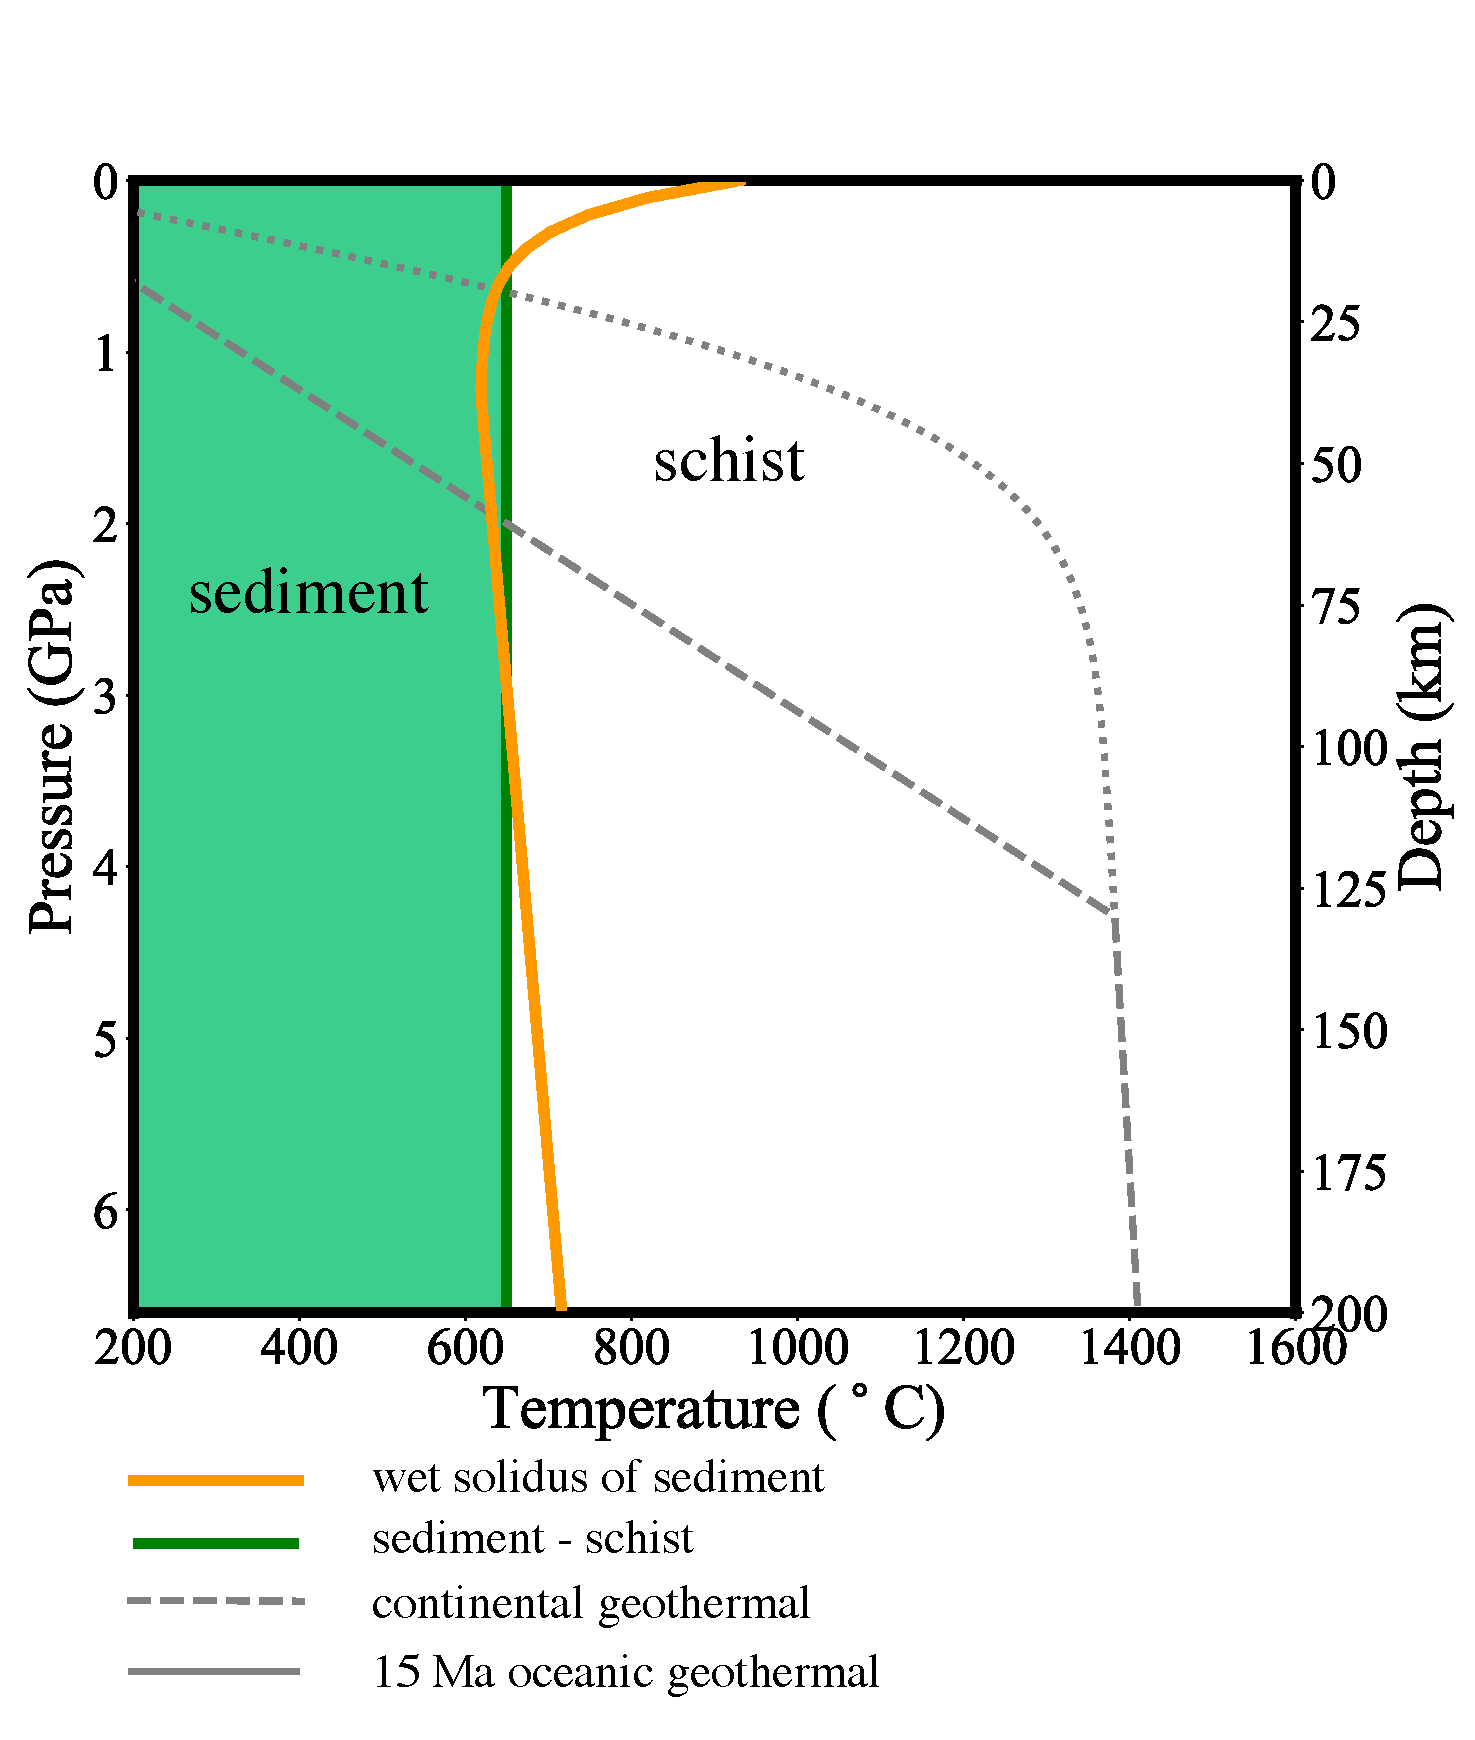
\includegraphics[width=4in]{sediment_phase_diagram_v1.pdf}
    \caption[沉積物變質岩相圖,參考自\citealp{van2011subduction}]{沉積物變質岩相圖,橘線為沉積物含水固相線,參考自\citealp{van2011subduction}。}
    \label{fig::sediment_phase_diagram}
\end{figure*}

\subsection{含綠泥石之橄欖岩 --- 橄欖岩}

模型中的地函除了普通橄欖石與蛇紋化橄欖石之外,還有考慮含綠泥石之橄欖岩的存在。
本研究假設部分熔融事件只會發生在具有含綠泥石之橄欖岩的海洋岩石圈上方的地函楔。
一旦溫度太高而使岩石脫水,含綠泥石之橄欖岩就會轉變為一般的橄欖石。
相變條件式參考自\citealp{Grove2009},簡化式如下:
\begin{align}
T > 800-3.5\times 10^{-8}\times (P\times 3 \times 10^{4} -62)^{2 \;\circ}C
\end{align}
其中$P$為十億帕斯卡(GPa)。
圖\ref{fig::chlorite_phase_diagram}為含綠泥石之橄欖岩岩相圖。
\begin{figure*}[ht!]
    \centering
    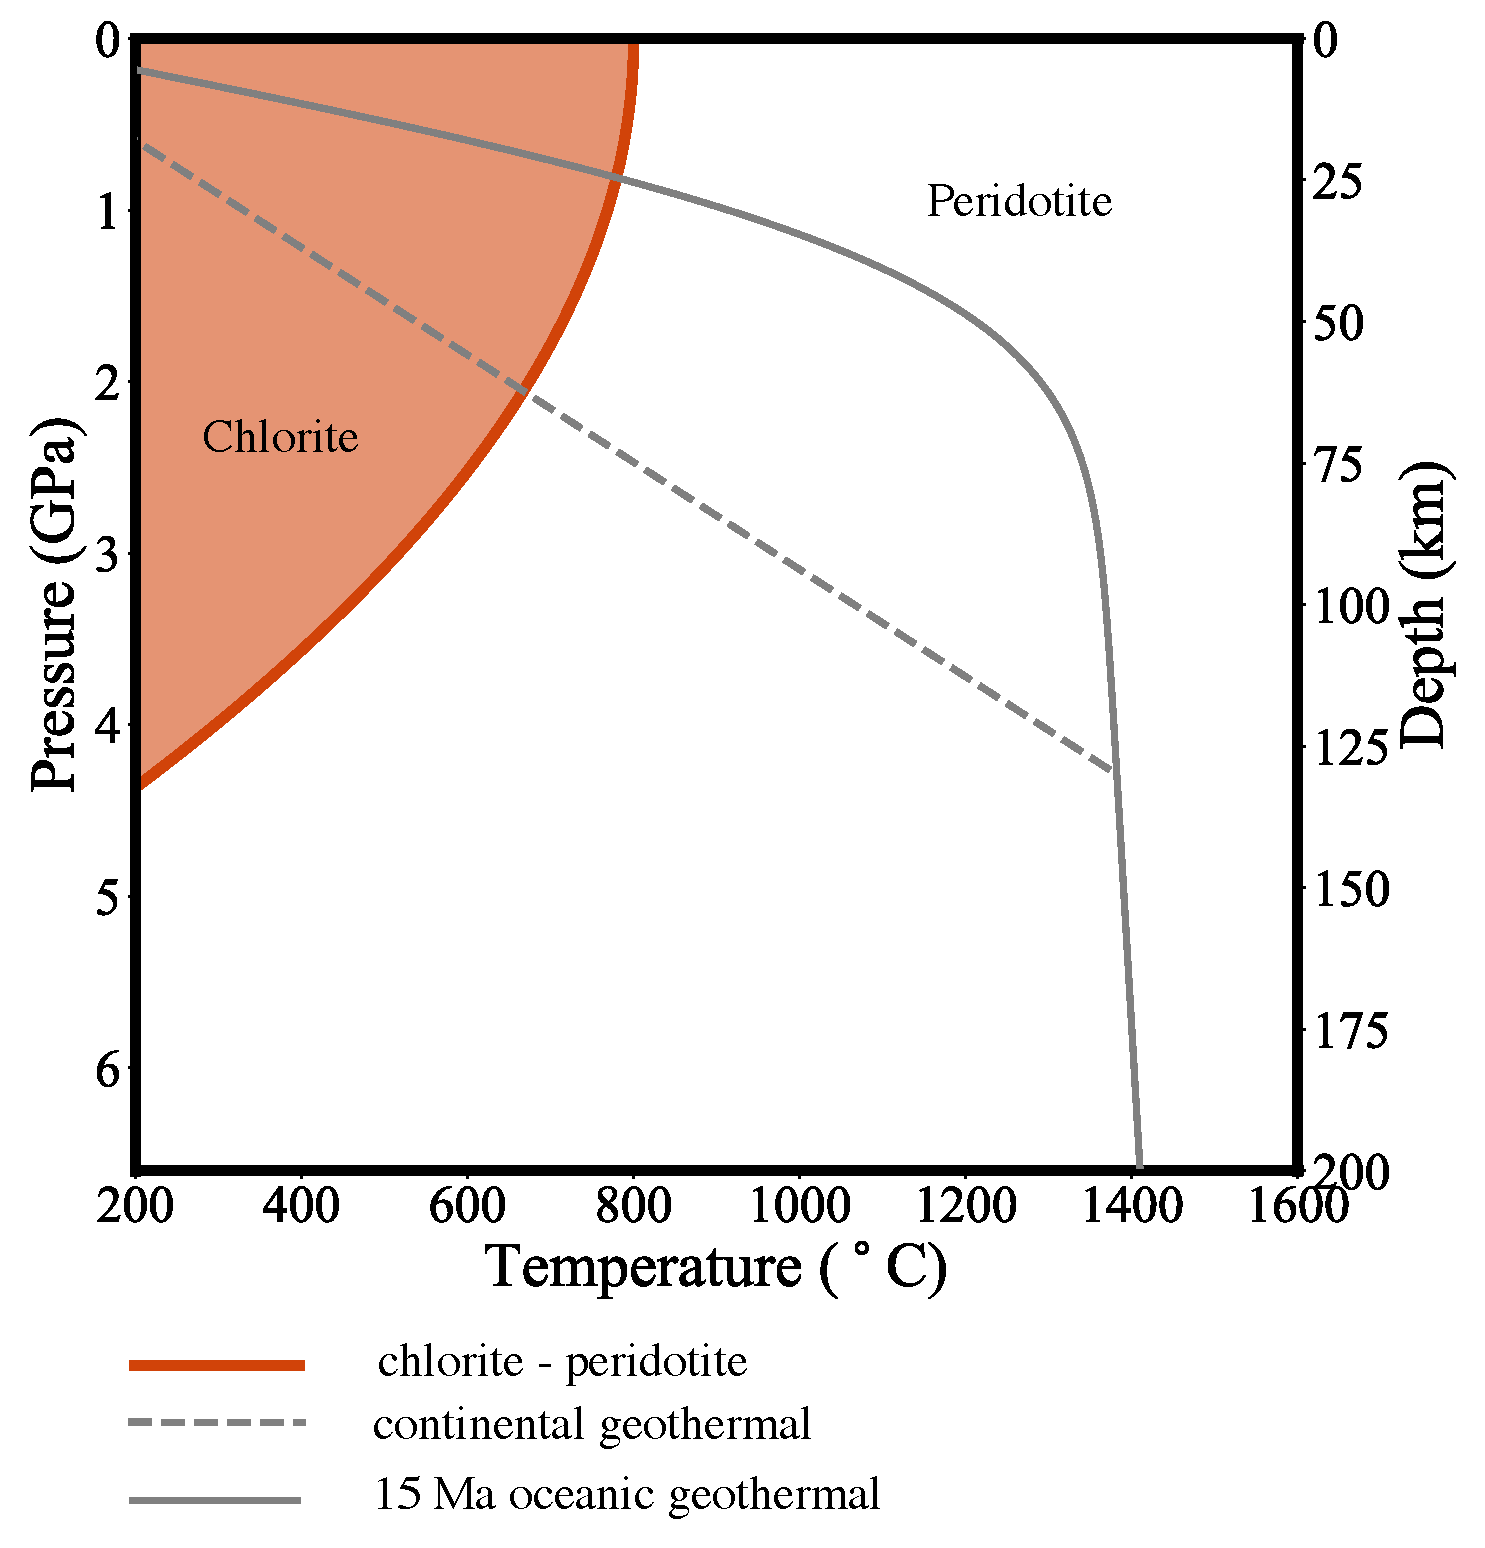
\includegraphics[width=4in]{chlorite_phase_diagram_v1.pdf}
    \caption[含綠泥石之橄欖岩岩相圖,參考自\citealp{Grove2009}]{含綠泥石之橄欖岩岩相圖,橘紅線為含綠泥石之橄欖岩脫水相變線,參考自\citealp{Grove2009}。}
    \label{fig::chlorite_phase_diagram}
\end{figure*}

\section{熱邊界條件}\label{熱邊界條件}
%\subsection{運動邊界條件}
%在現實自然界中,板塊水平移動的主要作用力為板塊拉力和洋脊推力兩個分量,
%為了方便控制隱沒系統的聚合速度,本研究數值模型會對模型邊界施加速度控制隱沒系統的聚合速度,此為模型運動邊界條件。
%而模型中板塊主要的驅動力則由運動邊界條件所施加的速度控制。

%於本研究中所使用的板塊水平移動運動起初由速度邊界條件所決定,在模型運算期間皆為不隨時間變化的常數,然而,真實自然界中板塊移動速度與時間的關係不應為常數。
%在本研究的智利模型中,所使用的速度邊界條件滿足現生板塊移動速度模型(\citealp{schellart2008global})。然而在墨西哥模型中,由於其隱沒板塊較為年輕、強度低,在聚合速率較快的情況下容易發生海洋板塊斷裂的情況,因此
%因此在模型進行一段時間後,模型邊界條件隨邊界所承受之總體力大小所決定。

%模型會先設定左右邊界最大可施加的力臨界值大小Fc,當模型進行一萬個迴圈後,若邊界承受的力大於初始所給定的力臨界值,則會將速度下降為原先的0.9倍;反之若邊界承受的力尚未達到給定的力臨界值,則速度會增加為原先的1.1倍。此時,每一萬個迴圈,模型運動邊界條件會重新調整一次,以符合觀測結果。因此當模型運行一段時間之後,邊界所承受的力會約略相等於初始條件所設定的力臨界值。

%\subsection{熱邊界條件}\label{熱邊界條件}
本研究中海洋岩石圈溫度構造使用半空間冷卻模型(half space cooling model),海洋岩石圈厚度與岩石圈年紀之開根號呈正比。由 \citealp{davis1974}提出:
\begin{align}
T=T_0+(T_m-T_0)\cdot erf(\frac{z}{2\sqrt{\kappa t}}) \label{eq:Half Space Model}
\end{align}
$T$ 是溫度,$T_m$ 是地函溫度,在本研究中使用攝氏1330$^{\circ}$。
$z$ 是與地表的距離,單位是公里,$\kappa$ 是熱擴散系數,在本研究中使用$10^{-6} \frac{m}{s^2}$。$t$ 是海洋岩石圈年紀。

大陸板塊的溫度構造有雙層構造與單層構造之區別。
本研究根據墨西哥與智利過去的地球物理研究,分別對墨西哥模型與智利模型設定不同的大陸岩石圈溫度構造。

墨西哥模型中,大陸岩石圈為雙層構造,近地表每公里20度溫度梯度,直到深度至45公里之後溫度梯度為每公里6度,至溫度到達攝氏1330度後維持恆溫。
此溫度構造建立在過去墨西哥平坦隱沒區域溫度模型研究(\citealp{Manea2005}; \citealp{Manea2011Thermal}; \citealp{Manea2011Curie})所提供的約束。

智利模型中,大陸岩石圈地溫梯度是單層構造,以岩石圈底部深度140公里作為參考(\citealp{perez2008}),從地表攝氏0度到岩石圈底部攝氏1330度,中間進行線性內插,僅含單一地溫梯度,約略為每公里攝氏9.5度。

能量交換在岩石圈中以熱傳導為主,溫度變化極大,然而在軟流圈,熱能傳遞以對流為主,因此整個軟流圈至地函地核邊界(core mantle boundary)的溫度皆維持地函絕熱溫度,僅存在因密度變化所造成之絕熱溫度梯度,因此模型中將岩石圈底部溫度固定為地函絕熱溫度1330度。
不同構造區溫度隨深度變化圖見圖\ref{fig::geothermal}。
\begin{figure*}[ht!]
    \centering
    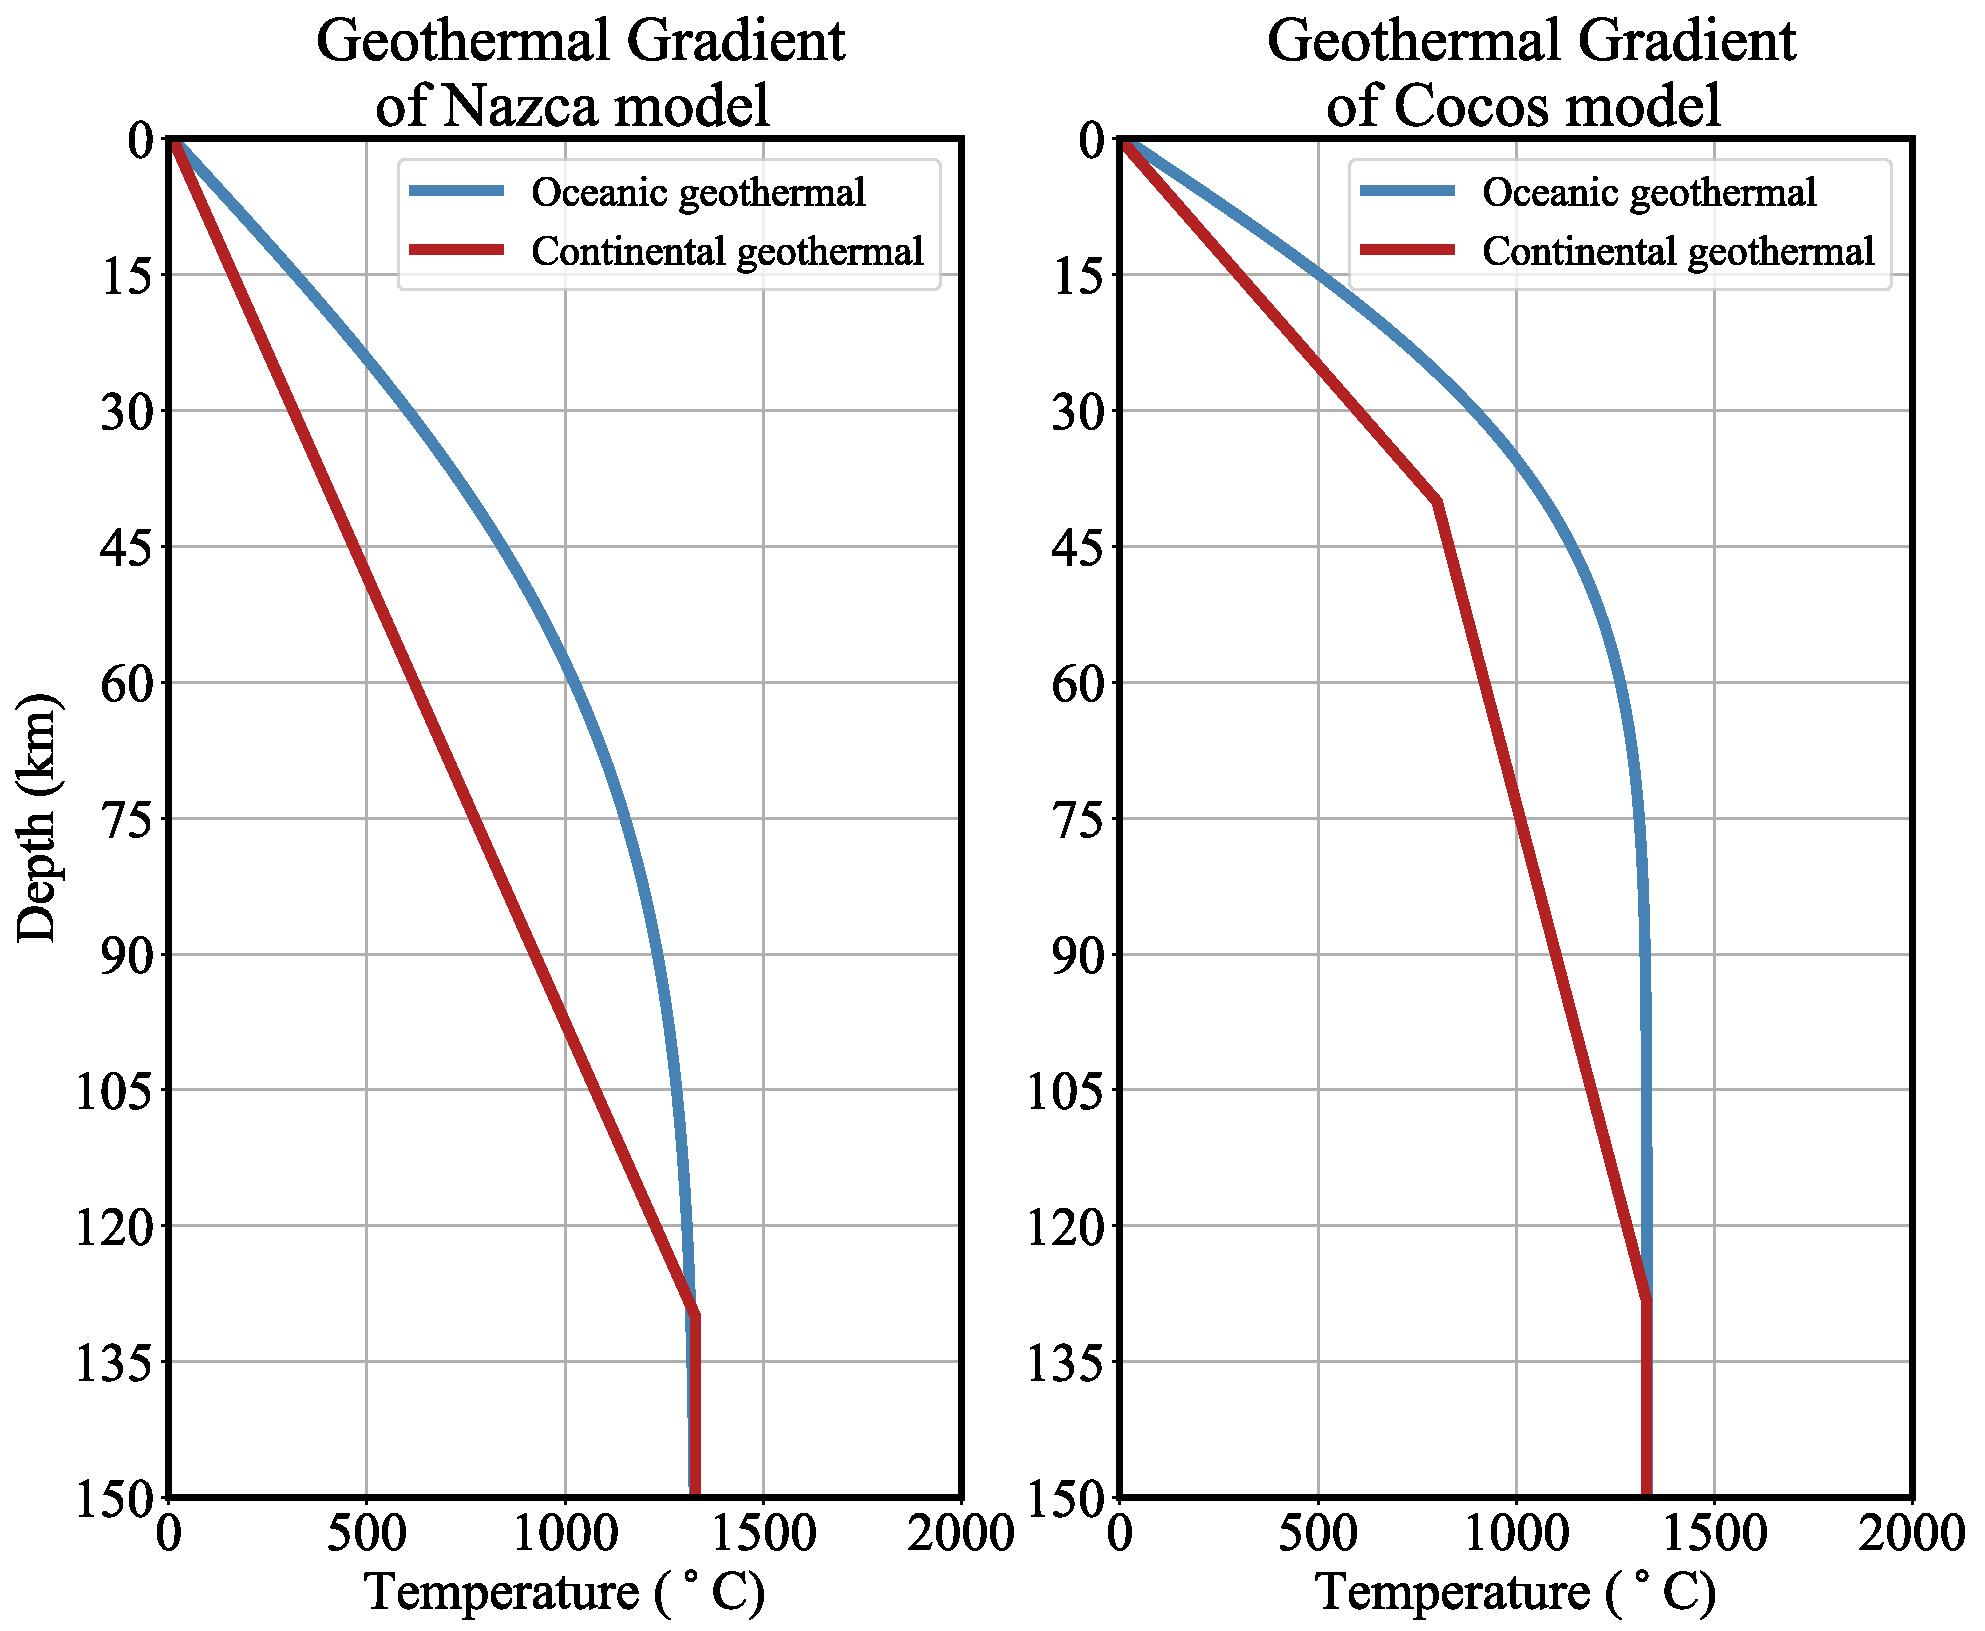
\includegraphics[width=5.5in]{temperature_profile_v2.pdf}
    \caption[本研究使用之模型地下溫度剖面圖]{本研究使用之模型地下溫度剖面圖,左圖為智利模型,右圖為墨西哥模型。藍色實線為海洋岩石圈地溫梯度,由式\ref{eq:Half Space Model}與海洋岩石圈年紀決定。咖啡色實線為大陸岩石圈地溫梯度,智利模型大陸岩石圈為單層構造,墨西哥模型大陸岩石圈為雙層構造。圖中並沒有考量絕熱地溫梯度。}
    \label{fig::geothermal}
\end{figure*}


\section{地表侵蝕}
地表地形演化與板塊構造活動有高度相關,在本研究模型中利用較簡單的方式模擬地形演化過程,包含侵蝕與沉積物堆積作用,使用一維擴散方程式控制侵蝕與堆積作用的速率,最早由\citealp{culling1960analytical} 所提出,其方程式如下:
\begin{align}
\frac{\partial z}{\partial t} = \kappa_S \nabla^2 z \label{eq:erosion}
\end{align}
其中$z$為模型中地表節點高度,其數學意義為對地表高度進行二次導數後得到該點曲率,並照曲率大小對其進行地形下修與上修,地形較突出處會被侵蝕,反之地形凹陷處容易被侵蝕物所堆積。物理意義則為守恆公式之展現,將地形假想為一二維空間方程式,在地形上每一點會因重力而有往下流動物質通量S,流動物質通量與地形坡度呈正比:
\begin{align}
\vec S = -k\nabla \vec z \label{eq:S}
\end{align}
其中$k$為正比係數。並且由於物質永遠守恆,在滿足守恆公式的假設下,物質質量不隨時間變化,令物質質量與時間的關係式:
\begin{align}
\rho\frac{\partial z}{\partial t}\label{eq:rho}
\end{align}

質量隨時間的變化會等同於物質在空間中的通量,因此式($\ref{eq:S}$) 與式($\ref{eq:rho}$) 的關係如下:
\begin{align}
\rho\frac{\partial z}{\partial t} = -\vec\nabla\cdot \vec S = -\vec\nabla \cdot (-k\nabla \vec z)\label{eq:erosion2}
\end{align}
或
\begin{align}
\frac{\partial z}{\partial t} = \frac{k}{\rho}\nabla^2 z\label{eq:erosion3}
\end{align}
令$\frac{k}{\rho}=\kappa_S$,其中$\kappa_S$為坡度擴散係數,本研究中侵蝕與堆積的坡度擴散係數相同,單位為$\frac{m^2}{s}$。可得:
\begin{align}
\frac{\partial z}{\partial t} = \kappa_S\nabla^2 z\label{eq:erosion4}
\end{align}

\section{岩漿作用}\label{岩漿作用}
本研究的數值模型包含隱沒帶中的岩漿作用。
隱沒板塊進入地函時,其上覆沉積物與玄武岩在進入高溫高壓環境的同時發生脫水與相變。
當水分進入地函楔中,其固相線(solidus)從乾固相線移動至含水固相線,隱沒板塊上方的橄欖岩熔點大幅降低。
地溫梯度因此容易經過含水固相線,發生部分熔融事件,隨後產生岩漿,部分岩漿分佈在地函與地殼中,成為岩漿庫(magma chamber),而剩餘岩漿噴發至地表形成火山島弧(volcanic arc)。

\begin{figure*}[ht]
    \centering
    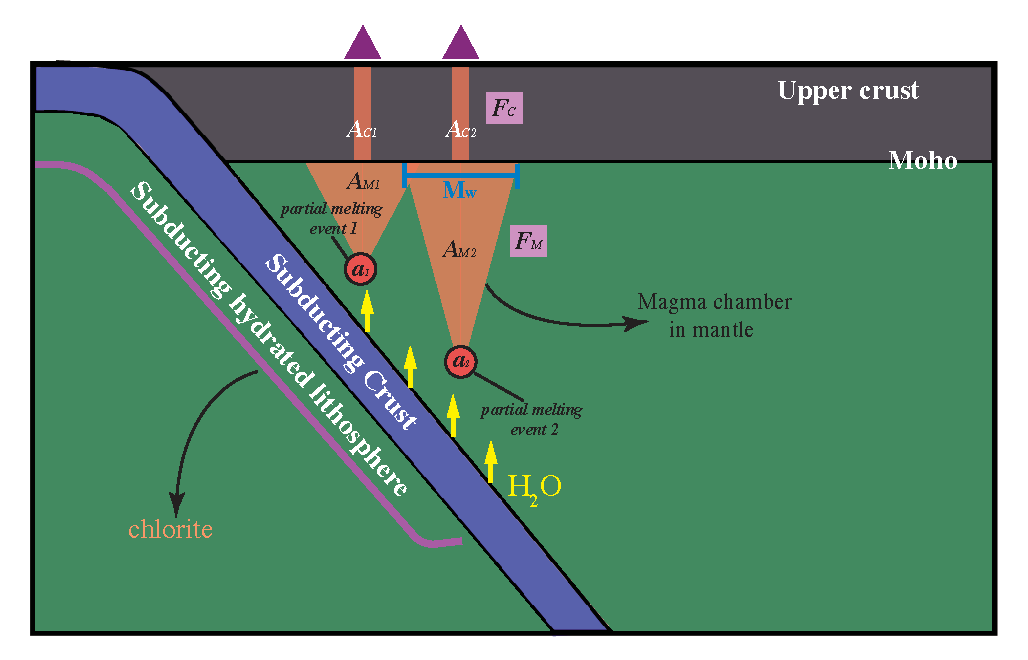
\includegraphics[width=6in]{melting.pdf}
    \caption[模型內岩漿作用示意圖。]{模型內岩漿作用示意圖。圖中繪製兩個不同的部分熔融事件。每個獨立部分熔融事件會對應獨立的岩漿庫。
    模型中有F$_M$比例的岩漿留在地函楔中,F$_C$比例的岩漿留在地殼中,其餘1-F$_M$-F$_C$比例的岩漿會噴發至地表形成火山島弧,如圖上方紅紫色三角形。
    地函岩漿庫中的岩漿均勻分布在圖中地函楔中紅橘色倒三角形。
    圖中假設部分熔融事件二的部分熔融體積為a$_2$地函岩漿庫體積為A$_{M2}$。
    }
    \label{fig::melting}
\end{figure*}

\subsection{部分熔融}\label{部分熔融}
本研究共考慮三種岩相的部分熔融,分別為在地函楔中的橄欖岩相(包含橄欖岩與蛇紋岩)、沉積岩相與鐵鎂質岩相(包含玄武岩與榴輝岩),並且假設最大部分熔融體積為總體網格內的10$\%$。
當上述三種岩相之標記點通過\ref{相變}節中提及之固相線後,便將該標記點視為熔融態,部分熔融比例($p_{melt}$)計算方式如下:
\begin{align}
    p_{melt}=\frac{(T-T_{solidus})}{500}\times 10\% \label{eq:melting}
\end{align}

其中$T_{solidus}$為該標記子深度下對應至固相線的溫度,即為熔點(melting point),部分熔融比例在熔點與高於熔點500度範圍內從0$\%$線性增加至10$\%$。
模型中允許多個部分熔融事件發生,並且會依照部分熔融比例累加,隨後藉由部分熔融比例計算模型中的岩漿量。

\subsection{岩漿庫}\label{岩漿庫}
本研究假設有F$_M$比例的岩漿留在地函楔中,F$_C$比例的岩漿留在地殼中,其餘1-F$_M$-F$_C$比例的岩漿會噴發至地表。
留在地函楔中的岩漿成為岩漿庫,部分熔融發生後,模型中假設從熔點開始產生一倒三角形的地函岩漿庫,假設地函岩漿庫頂部皆在莫荷面下,並在莫荷面處達到最大寬度$M_W$公里,如圖\ref{fig::melting}所示,該最大寬度與岩漿往左右移動的流動性有關,本研究中所有模型一律將最大寬度設為50公里。
由於本研究並沒有探討地殼中岩漿對模型動力的影響,因此地殼中的岩漿庫一律視為一垂直莫荷面的柱狀岩脈。

岩漿庫中每個網格的體積融化比例(M)為與時間相關的函數,每個部分熔融事件所產生的岩漿會在模型中累積。
每個時間點的體積融化比例分為每個時間點產生的岩漿量與每個時間點冷卻的岩漿量,由下式表示:
\begin{align}
    M(t+dt)-M(t) = \Delta M = Pdt-M(t)\lambda dt \label{eq:Magma}
\end{align}
\begin{align}
    P = P_0 \times p_{melt} \times F_M \times A \label{eq:Magma P}
\end{align}
\begin{align}
    \lambda = \lambda_0\times exp(-\lambda_T \times \Delta T) \label{eq:Magma lambda}
\end{align}
式\ref{eq:Magma}中,$Pdt$項為每時間點岩漿產生量,與部分熔融比例有關,$P$為岩漿產生速率。
$M(t)\lambda dt$為每時間點岩漿冷卻量(岩石結晶量),與岩漿庫大小有關,$\lambda$為岩漿冷卻速率。
式\ref{eq:Magma P}計算岩漿產生速率,$P_0$是岩漿產生常數,單位為$m^3/m/s$,亦即每海溝截面所產生的岩漿體積速率。
$p_{melt}$來自式\ref{eq:melting},為部分熔融百分比。
A為發生部分熔融的體積比例,地函中的A為發生部分熔融體積與預設岩漿庫倒三角形的總面積比值,以圖\ref{fig::melting}的部分熔融事件二而言,A = (部分熔融發生面積 a$_2$/倒三角形面積 A$_{M2}$);地殼中的A = (部分熔融發生面積a$_2$/地殼岩脈面積A$_{C2}$)。
$\Delta T$為包含岩漿的網格與周遭網格的溫度差,溫度差越高(亦即周遭網格溫度越低),則岩漿冷卻速率越快。
式\ref{eq:Magma lambda}描述岩漿冷卻參數$\lambda$,$\lambda_0$為岩漿冷卻衰變常數,$\lambda_T$是與溫度有關的冷卻係數,單位為$\frac{1}{K}$。

岩漿量的變化意味著岩石的物態改變。
物質的物態改變在溫度相同的情形下會有能量的吸收或釋放,本研究有考慮岩漿量變化過程中的能量變化。
\subsection{岩漿作用造成的溫度影響}\label{岩漿作用造成的溫度影響}
本研究只考慮在岩漿結晶過程中所釋放的潛熱(放熱)。
模型中會計算每個時間的岩漿變化量($\Delta M$),估計岩漿結晶冷卻中釋放的能量與其所造成的溫度變化量,使用公式如下:
\begin{align}
    T(t+dt) = T(t) + M(t+dt)\times \lambda \times dt \times \frac{L_H}{C_p}\label{eq:latent heat}
\end{align}
其中$L_H$為岩漿潛熱值,在本研究使用安山岩漿的潛熱值$3\times 10^5$ J/kg(\citealp{liu2011modeling})。
$C_p$為等壓比熱容量。

當岩漿結晶後,周遭岩石的溫度因放熱而有局部升高的現象,該過程會些微影響地函楔中的黏滯度與隱沒帶動力過程。

\section{計算數值模型中的轉動力矩}\label{計算數值模型中的轉動力矩}
本研究利用數值解的結果計算模型中不同時間點,在假設海溝為支點的情況下,獲得隱沒板塊所受的重力力矩與動水壓力力矩。
本研究所使用重力力矩數值求解式如下:
\begin{align}
    \tau_{gravity} =  g\sum ^L_{l=0} \Delta \rho(l)\ r(l)\ cos\ \alpha (l)\ V(l) 
    \label{eqn:tau_gravity}
\end{align}
整段隱沒板塊被切割成$l$段板塊,每段$l$皆有個別的密度差$\Delta \rho(l)$、力臂(moment arm)為$r(l)\ cos\ \alpha (l)$與體積$V(l)$。
其中$r(l)$為從支點到$l$段中心點的直線距離,$ \alpha (l)$為$r(l)$與重力的夾角,亦即$r(l)$與垂直方向上的夾角,固$r(l)\times cos\ \alpha (l)$為轉動系統中的力臂。體積$V(l)$由隱沒板塊上攝氏800$^{\circ}$等溫線以內範圍所決定。

本研究所使用動水壓力力矩數值求解式如下:
\begin{align}
    \tau_{suction} =  \sum ^L_{l=0} [P_{sub}(l)-P_{wedge}(l)]\cdot dl \cdot cos\ \beta(l)\cdot r(l)\ 
    \label{eqn:tau_suction}
\end{align}
與重力力矩計算方法雷同,將隱沒板塊切割成$l$段,計算直接垂直於每段$l$上下的模型動態壓力差與$dl$段的乘積獲得作用在隱沒板塊上的壓力梯度力,並且再乘上$dl$段與力臂的夾角$\beta(l)$獲得作用力於力矩上的實際大小。
最後計算壓力梯度力與力臂的乘積便為每段$l$所受的動水壓力力矩。

積分每段$l$所造成的轉動重力力矩與動水壓力力矩後便可得該時間點下的總重力力矩與總動水壓力力矩,由於本研究為二維模型,單位皆為N$\cdot$ m/m。


\begin{landscape}
\begin{table}[htp]\large
    \caption[模型中岩石參數列表,參考自\citealp{ranalli1995rheology}]{模型中岩石參數列表,參考自\citealp{ranalli1995rheology}。}
    \renewcommand{\arraystretch}{1.5}
    \begin{tabular}{m{5.5cm}m{2cm}m{2cm}m{2.4cm}m{2.3cm}m{1cm}m{1cm}m{1.7cm}m{1.7cm}}
        \hline
        Material                                                                                    & \begin{tabular}[c]{@{}l@{}}Density\\ (kg m$^{-3}$)\end{tabular} & n    & \begin{tabular}[c]{@{}l@{}}A\\ (MPa$^{-n}$s$^{-1}$)\end{tabular} & \begin{tabular}[c]{@{}l@{}}E\\ J$\cdot$ m\textasciicircum{}\{-3\}\end{tabular} & \begin{tabular}[c]{@{}l@{}}$\phi_0$\\ ($^{\circ}$)\end{tabular} & \begin{tabular}[c]{@{}l@{}}$\phi_1$\\ ($^{\circ}$)\end{tabular} & \begin{tabular}[c]{@{}l@{}}$C_0$\\ Pa\end{tabular} & \begin{tabular}[c]{@{}l@{}}$C_1$\\ Pa\end{tabular} \\ \hline
        basalt                                                                                      & 2880                                                            & 3.05 & 1.25$\times$10$^{-1}$                                                          & 3.76$\times$10$^5$                                                                         & 30                                                              & 15                                                              & 4$\times$10$^7$                                                & 4$\times$10$^6$                                                 \\
        eclogite                                                                                    & 3480                                                            & 3.05 & 1.25$\times$10$^{-1}$                                                          & 4.5$\times$10$^5$                                                                          & 30                                                              & 15                                                              & 4$\times$10$^7$                                                & 4$\times$10$^6$                                                 \\
        continental upper crust                                                                     & 2800                                                            & 3.05 & 1.25$\times$10$^{-1}$                                                          & 2.76$\times$10$^5$                                                                         & 30                                                              & 15                                                              & 4$\times$10$^7$                                                & 4$\times$10$^6$                                                 \\
        \begin{tabular}[c]{@{}l@{}}continental lower crust/ arc\\ (strong lower crust)\end{tabular} & 2900                                                       & 3.05 & 1.25$\times$10$^{-1}$                                                          & 5.76$\times$10$^5$                                                                         & 30                                                              & 15                                                              & 4$\times$10$^7$                                                & 4$\times$10$^6$                                                 \\
        \begin{tabular}[c]{@{}l@{}}continental lower crust \\ (weak lower crust)\end{tabular}       & 2900                                                            & 3.05 & 1.25$\times$10$^{-1}$                                                             & 2.76$\times$10$^5$                                                                         & 30                                                              & 15                                                              & 4$\times$10$^7$                                                & 4$\times$10$^6$                                                 \\
        sediment                                                                                    & 2800                                                            & 3    & 5$\times$10$^2$                                                              & 2$\times$10$^5$                                                                            & 3                                                               & 3                                                               & 4$\times$10$^6$                                                & 4$\times$10$^6$                                                 \\
        schist                                                                                      & 2900                                                            & 3    & 7$\times$10$^4$                                                              & 3.76$\times$10$^5$                                                                         & 30                                                              & 15                                                              & 4$\times$10$^7$                                                & 4$\times$10$^6$                                                 \\
        mantle (perdiotite)                                                                         & 3300                                                            & 3    & 7$\times$10$^4$                                                              & 5.2$\times$10$^5$                                                                          & 30                                                              & 15                                                              & 4$\times$10$^7$                                                & 4$\times$10$^6$                                                 \\
        serpentinite                                                                                & 3200                                                            & 3    & 7$\times$10$^4$                                                              & 1.2$\times$10$^5$                                                                          & 3                                                               & 3                                                               & 4$\times$10$^6$                                                & 4$\times$10$^6$                                                 \\
        chlorite                                                                                    & 3300                                                            & 3    & 7$\times$10$^4$                                                              & 5.2$\times$10$^5$                                                                          & 30                                                              & 15                                                              & 4$\times$10$^7$                                                & 4$\times$10$^6$                                                 \\ \hline
    \end{tabular}
\label{table::phase_table}
\footnotesize 所有岩石的熱傳導係數(thermal conductivity) = 3.3 Wm$^{-1}$$^{\circ}$C$^{-1}$,比熱容(heat capacity) = 10$^3$J $\cdot$kg$^{-1} \cdot$ K$^{-1}$,熱膨脹係數(thermal expansion) = 5 $\times$ 10 $^{-5}$ K $^{-1}$
\end{table}
\end{landscape}